% !TeX spellcheck = de_DE
%% 
%% This is file 'beamer_sample.tex'
%% 	
%% by Mathias Winkel
%%
%% Problems, bugs and comments to 
%% mathias.winkel2@uni-rostock.de
%%
\RequirePackage{fix-cm} % because of font size substituion warnings
\documentclass[10pt]{beamer} % die 10pt sollten festgelegt bleiben, da dies die Groesse der Mathematikschrift etc. beeinflusst

\usepackage[ngerman]{babel}  % deutsche Bezeichnungen und Trennung etc
\usepackage[utf8]{inputenc}
\usepackage[T1]{fontenc}
\usepackage{csquotes}
\usepackage{hyperref}        % interne Hyperlinks
\usepackage[scaled]{beramono}
\usepackage{microtype}
\usepackage{listings}
\usepackage{ragged2e}
\usepackage{marvosym}
\usepackage{xcolor}
\usepackage{pgffor}

%******************************************
% For giving image sources, see http://tex.stackexchange.com/a/48485
\usepackage[absolute,overlay]{textpos}
\setbeamercolor{framesource}{fg=gray}
\setbeamerfont{framesource}{size=\tiny}

\setbeamercolor{plain}{fg=black,bg=white}

\newcommand{\source}[1]{\begin{textblock*}{4cm}(8.2cm,8.6cm)
		\begin{beamercolorbox}[ht=0.5cm,right]{framesource}
			\usebeamerfont{framesource}\usebeamercolor[fg]{framesource} Quelle: {#1}
		\end{beamercolorbox}
	\end{textblock*}}
%******************************************

\lstdefinestyle{customc}{
	tabsize=2,
	belowcaptionskip=1\baselineskip,
	breaklines=true,
	xleftmargin=\parindent,
	language=C,
	showstringspaces=false,
	basicstyle=\scriptsize\ttfamily,
	keywordstyle=\bfseries\color{green!40!black},
	commentstyle=\itshape\color{purple!40!black},
	identifierstyle=\color{blue},
	stringstyle=\color{orange},
}

\lstset{escapechar=@,style=customc}

\definecolor{links}{HTML}{2A1B81}
\hypersetup{colorlinks,linkcolor=,urlcolor=structure.fg}

\newcommand{\framefrompdf}[2]{
	\begin{frame}[plain]
		\hspace*{-8.5pt}
		\begin{beamercolorbox}[wd=\paperwidth,ht=\paperheight]{plain}
			\makebox[\paperwidth]{\hspace{8.5pt}\includegraphics[page=#2,width=\paperwidth]{#1}}
		\end{beamercolorbox}
	\end{frame}
}

\newcommand{\framesfrompdf}[3]{
	\foreach \n in {#2,...,#3}{\framefrompdf{#1}{\n}}
}

\newcommand{\framesfrompdfclipped}[8]{
	\foreach \n in {#2,...,#3}{
		\begin{frame}[plain]
			\vspace*{-18pt}\hspace*{-8.5pt}
			\makebox[\linewidth]{\includegraphics[page=\n,width=#8,clip,trim = #4 #5 #6 #7]{#1}}
		\end{frame}
	}
}

\newcommand{\picturefrompdf}[7]{
	\begin{center}
		%trim option's parameter order: left bottom right top
		\includegraphics[page=#2,width=#7,clip,trim = #3 #4 #5 #6]{#1} 
	\end{center}
}

\newcommand{\rto}{$\Rightarrow$ }

\newcommand{\emp}[1]{{\color{orange}{#1}}}

\newcommand{\img}[2]{
	\centering
	\includegraphics[#2]{figures/#1}
}

\newcommand{\questions}{
\begin{frame}
	
	\centering
	\Large
	Fragen?

\end{frame}
}

\newenvironment{task}[1]{
	\begin{block}{\textbf{Aufgabe} \hfill #1}
}{
	\end{block}
}

\AtBeginSection[]
{
	\begin{frame}{Plan für heute}
		\tableofcontents[currentsection]
	\end{frame}
}

\usepackage[uni,footuni,headlogo]{./unirostock/beamerthemeRostock}
% erster Parameter: Farbschema
%        moegliche Werte (nomen est omen): uni, inf, msf, ief, mnf, mef, juf, wsf, auf, thf, phf
%        Standardwert: uni
% zweiter Parameter: Fusszeile
%        moegliche Werte: footuni (Standard) - Fusszeile nach Handbuch des CD
%                         foottitle          - Autor und Title in der Fusszeile
%                         footheadings       - lebende Ueberschriften in der Fusszeile
%                         footuniheadings    - Autor und Uni sowie lebende Ueberschriften in der Fusszeile
% dritter Parameter: Kopfzeile
%        moegliche Werte: headlogo (Standard)- Inhalt von \mylogo in der Kopfzeile
%                         headtitle          - Vortragstitel
%                         headframetitle     - Folientitel
%                         headframesubtitle  - Folientitel und -untertitel
%        bitte nicht mehrere Varianten gleichzeitig angeben :-)

\setbeamercovered{invisible}
\addtobeamertemplate{block begin}{}{\justifying}

%%%%%%%%%%%% Festlegung der Titelseite %%%%%%%%%%%%%%%%%%%%%%%%%%%%%%%%%
\title[]{Imperative Programmierung}

\subtitle{Übung}

\author{\textsc{Tom Warnke}}

\institute{Universität Rostock, Institut für Informatik}

\titlegraphic{}

% ein alternatives Titelbild kann mittels 
%\titleimage{Dateiname.xyz}
% angegeben werden (auf vernuenftiges Seitenformat und Kontrastwerte achten, Skalierung und Abschneiden der oberen rechten Ecke passieren automatisch)
\titleimage{}

%%%%%%%%%%%% Festlegungen fuer Kopf- und Fusszeile %%%%%%%%%%%%%%%%%%%%
% Institutsname f\"ur die Fusszeile (nur wenn bei Paketeinbindung 'footuni' angegeben ist)
\footinstitute{Fakultät für Informatik und Elektrotechnik, Institut für Informatik}
% eigenes Logo oben rechts hinzufuegen (bitte auf vernuenftiges Format achten - ein zu hohes Logo verschiebt das Layout)
\renewcommand{\mylogo}{}

%%%%%%%%%%%%%%%%%%%%%%%%%%%%%%%%%%%%%%%%%%%%%%%%%%%%%%%%%%%%%%%%%%%%%%%

\date{} % Hier kann das Datum des Vortrages festgelegt werden (fuer Fusszeile etc.)

%%%%%%%%%%%%%%%%%%%%%%%%%%%%%%%%%%%%%%%%%%%%%%%%%%%%%%%%%%%%%%%%%%%%%%%
\begin{document}

\maketitle  

\begin{frame}{Plan für heute}

	\tableofcontents

\end{frame}

\section{Grammatiken}

\begin{frame}{Grammatiken}
	
	\begin{itemize}
		\item Grammatiken beschreiben eine Sprache, indem sie vorschreiben, wie die \enquote{Worte} der Sprache gebildet werden.
		\item Nonterminale werden nach Vorschriften durch Terminale ersetzt
		\item EBNF - Produktionsregeln zum Einsetzen
		\item Syntaxdiagramme - Graph zum Ablaufen
	\end{itemize}
	
\end{frame}

\begin{frame}[fragile]{Grammatik von C}
	
	\texttt{if}-Anweisung als EBNF und Syntaxdiagramm:
	
	\vspace{2ex}
	
	\img{c-syntax-cropped}{width=\textwidth}
	
	\begin{lstlisting}[gobble=2,language=]
	<selection-statement> ::= if ( <expression> ) <statement>
	                        | if ( <expression> ) <statement> else <statement>
	\end{lstlisting}
	
	\source{
		\href{http://www.cs.utsa.edu/~wagner/CS2213/resources/C_reference.pdf}{XL C Language Reference} \&
		\href{https://cs.wmich.edu/~gupta/teaching/cs4850/sumII06/The\%20syntax\%20of\%20C\%20in\%20Backus-Naur\%20form.htm}{cs.wmich.edu}
	}
	
\end{frame}

\section{Struktogramme}

\begin{frame}{Struktogramme}{a.k.a. Nassi-Shneiderman-Diagramme}

	Eine Möglichkeit, Algorithmen zu beschreiben
	
	\begin{center}
		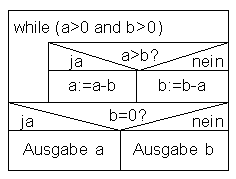
\includegraphics[width=0.4\linewidth]{figures/NassiShneiderman.png}
	\end{center}
	
	\source{\href{https://de.wikipedia.org/wiki/Nassi-Shneiderman-Diagramm}{Wikipedia}}

\end{frame}

\section{Variablen \& Ein- und Ausgabe}

\begin{frame}{Variablen in \texttt{C} speichern Werte}

	\begin{itemize}
		\item Variablen haben immer einen \emp{Namen}, einen \emp{Typ} und einen \emp{Wert}
		\item Es gibt verschiedene Datentypen in \texttt{C}
		\item Jeder Datentyp hat einen Wertebereich und Platzbedarf
	\end{itemize}
	
	\vspace{3ex}
	
	\begin{columns}
		\begin{column}{0.15\linewidth}
			 Deklaration\\\lstinline|int a;|
		\end{column}
		\begin{column}{0.15\linewidth}
			Wertzuweisung\\\lstinline|a = 5;|
		\end{column}
		\begin{column}{0.4\linewidth}
			Deklaration und Wertzuweisung\\\lstinline|int a = 5;|
		\end{column}
	\end{columns}

\end{frame}

\begin{frame}{Eine Auswahl von Datentypen}

	\begin{tabular}{|c|c|c|c|}
		\hline Datentyp & Inhalt & Wertebereich & Speicherplatz \\ \hline
		\hline \lstinline{int} & Ganze Zahl & -2,147,483,648 .. 2,147,483,647 & 32 Bit \\ 
		\hline \lstinline{char} & ASCII-Zeichen & 0 .. 255 (= a .. z, A .. Z, etc.) & 8 Bit \\ 
		\hline \lstinline{float} & Fließkommazahl & -3.4E38 .. 3.4E38 & 32 Bit \\ 
		\hline \lstinline{double} & Fließkommazahl & -1.7E308 .. 1.7E308 & 64 Bit \\ 
		\hline 
	\end{tabular} 

\end{frame}

\begin{frame}[fragile]{Eingabe und Ausgabe mit \lstinline{scanf} und \lstinline{printf}}
	
	\begin{itemize}
		\item Um einen Wert mit \lstinline{printf} auszugeben oder mit \lstinline{scanf} einzulesen, wird ein Platzhalter verwendet
		\begin{itemize}
			\item[\%d] Ganze Zahl
			\item[\%f] Fließkommazahl
			\item[\%c] Zeichen
		\end{itemize}
		\item Echo für ganze Zahlen:
			\begin{lstlisting}[gobble=8]
				int num;              /* Variable deklarieren */
				scanf("%d", &num);    /* Wert einlesen */
				printf("%d", num);    /* Wert ausgeben */
			\end{lstlisting}
		
	\end{itemize}	
	
\end{frame}

	% end of presentation
	%%%%%%%%%%%%%%%%%%%%%%%%%%%%%%%%%%%%%%%%%%%%%%%%%%%%%%%%%%%%%%%%%%%%%%%
	% backup slides
	
	\appendix
	\newcounter{finalframe}
	\setcounter{finalframe}{\value{framenumber}}
	
	%%%%%%%%%%%%%%%%%%%%%%%%%%%%%%%%%%%%%%%%%%%%%%%%%%%%%%%%%%%%%%%%%%%%%%%
	% end of backup slides
	\setcounter{framenumber}{\value{finalframe}}
\end{document}

